\documentclass[aps,floatfix,11pt]{revtex4-1}
\usepackage{bm}%bold math
\usepackage{graphicx}
\usepackage{amsmath}
\usepackage{amssymb}
\usepackage{setspace}
\linespread{1}

\begin{document}

\title{Notes}

\date{\today}

\begin{abstract}
    
\end{abstract}

\maketitle 

\section{Moves and Rules}

Creating a pair of stars in the staggered state is shown in fig. \ref{fig:create_pair}. We notice
the creation of a star produces two flippable plaquettes between the two stars.

\begin{figure}[h]
    \centering
    \includegraphics[width=8.5 cm]{create_pair}
    \caption{The creation of a pair of stars in the fully packed staggered configuration. The red
    dots on the $x$ and $y$ axes show the dimer about which the stars are created.
\label{fig:create_pair}}
\end{figure}

\noindent In fig. \ref{fig:move_right} we show the rightmost star move right in the same
configuration. In any single star must remain on the sublattice it was created on, so the center of
the star moves by two vertices. We notice that the horizontal propagation of a star creates two boundaries of
flippable plaquettes across the top and bottom of the star pair. 

\begin{figure}[h]
    \centering
    \includegraphics[width=8.5 cm]{move_right}
    \caption{The move of the rightmost star in fig. \ref{fig:create_pair} \label{fig:move_right}}
\end{figure}

Still figuring out the possible ways to move stars vertically. In six steps we show it is possible
to implement a specific type of local vertical move. 
\\

\begin{itemize}
    \item 
    Step 1 (fig. \ref{fig:ex_vert_mv_1}): create a pair of stars.
    
    \item 
    Step 2 (fig. \ref{fig:ex_vert_mv_2}): Move rightmost star right four times creating a horizontal set of
    flippable plaquettes.
    
    \item
    Step 3 (fig. \ref{fig:ex_vert_mv_3}): Flip some of the plaquettes. 
    
    \item
    Step 4 (fig. \ref{fig:ex_vert_mv_4}): With several vertical pairs of dimers we can flip on plaquette to make a
    horizontal pair that was not part of the original set of horizontal dimers after the star move. The
    $x$ and $y$ positions of this plaquette are marked in fig. \ref{fig:ex_vert_mv_4} by red dots along the $x$ and $y$
    axes. If all of the dimers were left as vertical or horizontal the move would not be possible.
    
    \item
    Step 5 (fig. \ref{fig:ex_vert_mv_5}): Create another pair of stars.
    
    \item
    Step 6 (fig. \ref{fig:ex_vert_mv_6}): Move the rightmost star of the new pair up. When this is done
    the dimers must be rearranged to satisfy the packing conditions and conserve the number of dimers.
    Right now this is the only configuration I see for this move that can satisfy these conditions.
\end{itemize}


\begin{figure}[h]
    \centering
    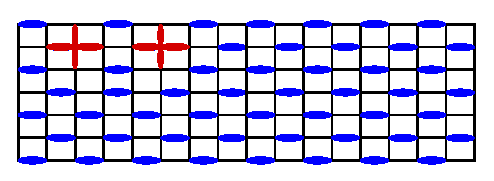
\includegraphics[width=8.5 cm]{ex_vert_mv_1}
    \caption{Step 1 in the vertical move example. Create a pair of stars.\label{fig:ex_vert_mv_1}}
\end{figure}

\begin{figure}[h]
    \centering
    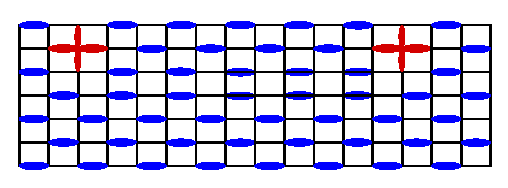
\includegraphics[width=8.5 cm]{ex_vert_mv_2}
    \caption{Step 2 in the vertical move example. Move the rightmost star right four times creating
    a horizontal set of flippable plaquettes.\label{fig:ex_vert_mv_2}}
\end{figure}

\begin{figure}[h]
    \centering
    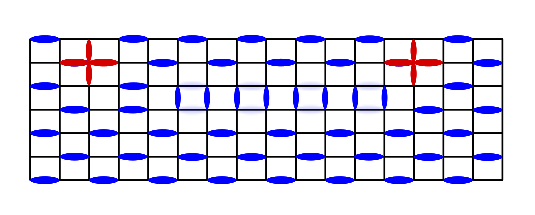
\includegraphics[width=8.5 cm]{ex_vert_mv_3}
    \caption{Step 3 in the vertical move example. Flip some of the plaquettes.\label{fig:ex_vert_mv_3}}
\end{figure}


\begin{figure}[h]
    \centering
    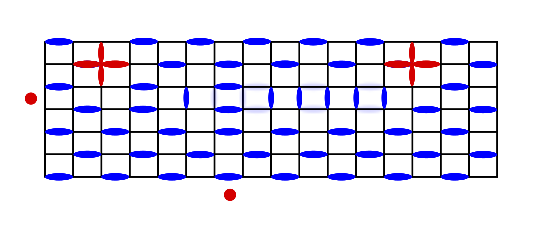
\includegraphics[width=8.5 cm]{ex_vert_mv_4}
    \caption{Step 4 in the vertical move example. Flip the plaquette at the $x$ and $y$ coordinates
    marked by the red dots.\label{fig:ex_vert_mv_4}}
\end{figure}


\begin{figure}[h]
    \centering
    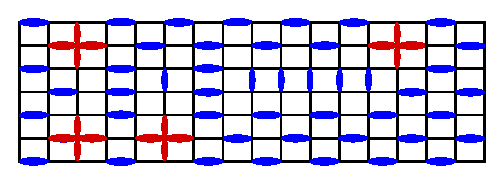
\includegraphics[width=8.5 cm]{ex_vert_mv_5}
    \caption{Step 5 in the vertical move example. Create another pair of stars.\label{fig:ex_vert_mv_5}}
\end{figure}

\begin{figure}[h]
    \centering
    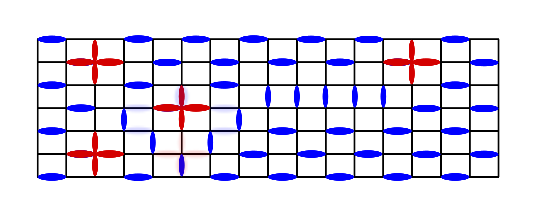
\includegraphics[width=8.5 cm]{ex_vert_mv_6}
    \caption{Step 6 in the vertical move example. Move the rightmost star of the new pair up.
    Rearrange the dimers around it to satisfy packing and conservation rules.\label{fig:ex_vert_mv_6}}
\end{figure}


% \bibliography{name_bib_file}

\end{document}
